
\begin{figure}
    \centering
    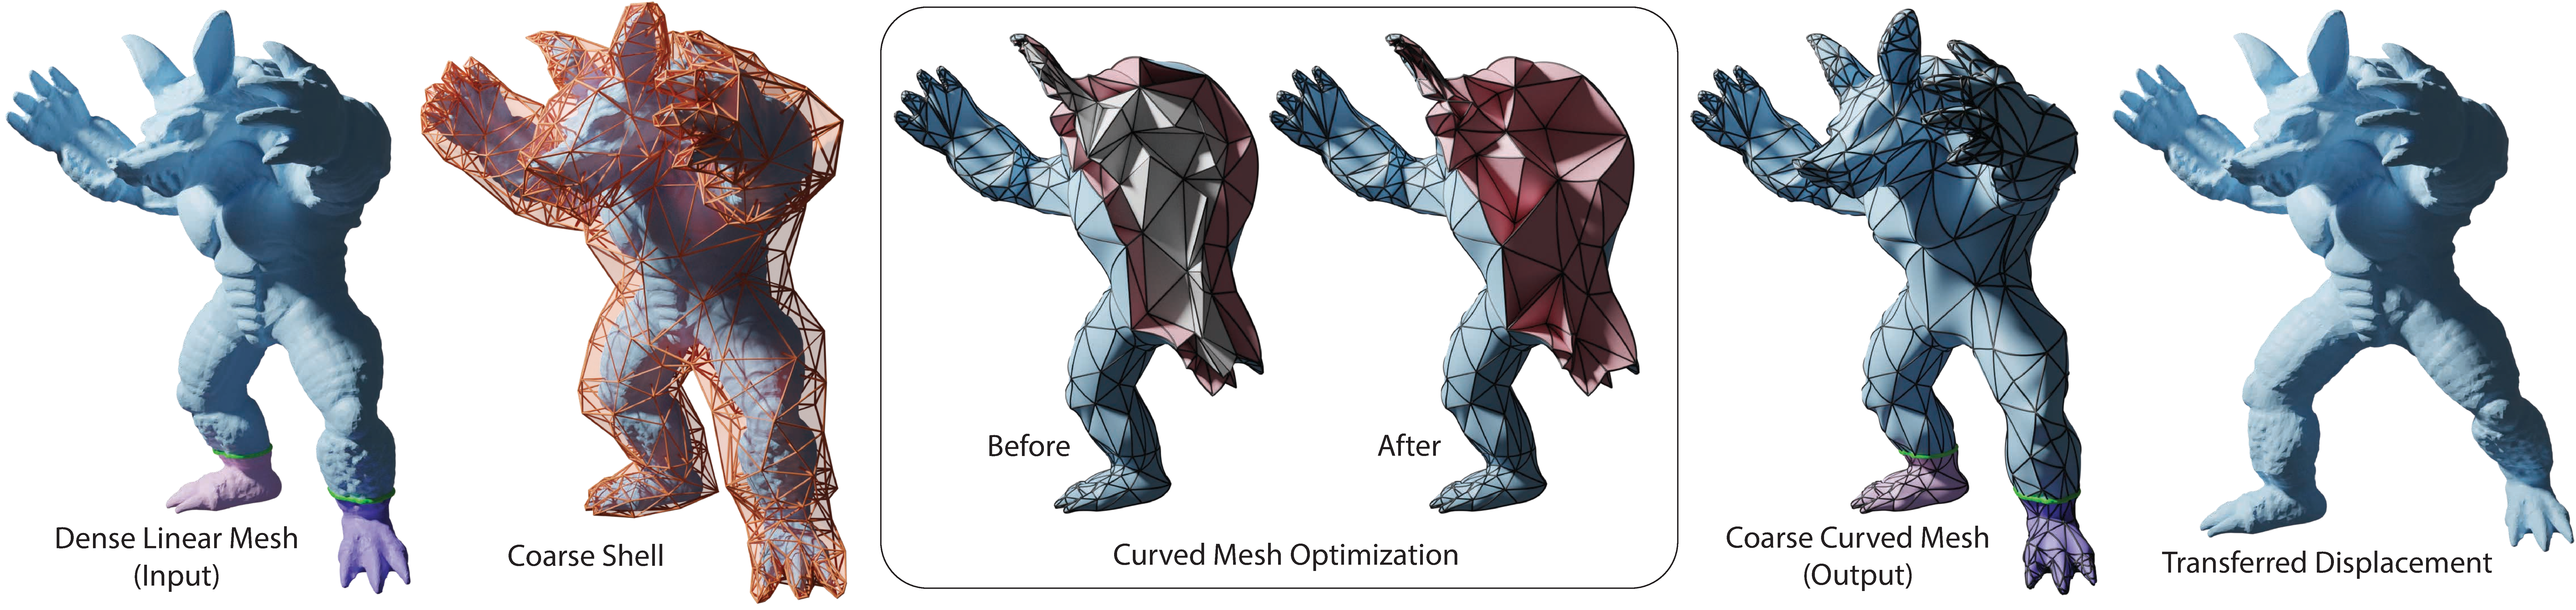
\includegraphics[width=\linewidth]{curve_meshing_in_shell_tex/figs/teaser}
    \caption{Our pipeline starts from a dense \emph{linear} mesh with annotated features (green), 
    which is converted in a curved shell filled with a high-order mesh. The region bounded by the shell is then tetrahedralized with linear elements, which are then optimized. Our output is a coarse, yet accurate, curved tetrahedral mesh ready to be used in FEM based simulation. Our construction provides a bijective map between the input surface and the boundary of the output tetrahedral mesh, which can be used to transfer attributes and boundary conditions.}
    \label{bichon:fig:teaser}
\end{figure}

\section{Introduction}

Piecewise linear approximations of surfaces are a popular representation for 3D geometry due to their simplicity and wide availability of libraries and algorithms to process them. However, dense sampling is required to faithfully approximate smooth surfaces. 
%
Curved meshes, that is, meshes whose element's geometry is described as a high-order polynomial, are an attractive alternative for many applications, as they require fewer elements to achieve the same representation accuracy of linear meshes. In particular, curved meshes have been shown to be effective in a variety of simulation settings in mechanical engineering, computational fluid dynamics, and graphics. Despite their major benefits, they are not as popular as linear meshes: We believe that {one of} the main reason for their limited usage is the lack of an automatic, robust way of constructing them. 

While robust meshing algorithm exists for volumetric linear tetrahedral meshing, there are few algorithms for curved meshes, and even fewer of them having either a commercial or open-source implementation (Section \ref{cumin:sec:related}). Only {a} few algorithms work directly on arbitrary triangle meshes (most of them require the input geometry to be either a CAD file or an implicit function), and none of them can reliably process a large collection of 3D models. 

We propose the first robust and automatic algorithm to convert dense piecewise linear triangle meshes (which can be extracted from scanned data, volumetric imaging, or CAD models) into coarse, curved tetrahedral meshes equipped with a bijective map between the input triangle mesh and the boundary of the tetrahedral mesh. Our algorithm takes advantage of the recently proposed bijective shell construction \cite{jiang2020bijective} to allow joint coarsening, remeshing, and curving of the dense input mesh, which we extend to support feature annotations.
Our outputs are guaranteed to have a self-intersection free boundary and the geometric map of every element is guaranteed to be bijective, an important requirement for FEM applications.

The key ingredient of our algorithm is the separation of the curved volumetric meshing problem into a near-surface, surface curving problem, followed by a restricted type of linear volumetric meshing. 


We believe that our curved meshing algorithm will enable wider adoption of curved meshes, as it will provide a way to automatically convert geometric data in multiple formats into a coarse tetrahedral mesh readily usable in finite element applications. To showcase the benefits of our approach we study 2 settings: (1) we show that a coarse proxy mesh can be used to compute non-linear deformations efficiently and transfer them onto a high-resolution geometry, targeting real-time simulation (Figure~\ref{bichon:fig:teaser}), and (2) 
we show that our meshes are ready to use in downstream FEM simulations.

We validate the reference implementation of our approach on a large collection of more than 8000 geometrical models, which will be released as an open-source project to foster the adoption of curved meshes in academia and industry.

Our contributions are:
\begin{itemize}
    \item An algorithm to convert dense piecewise linear meshes into coarse curved volumetric meshes while preserving a bijective map with the input and bounding the approximation error.
    \item An extension of the bijective shell construction algorithm to support feature {annotations}.
    \item An algorithm for conforming tetrahedral meshing without allowing refinement on the boundary, but allowing internal Steiner points.
    % \item A reusable open-source implementation of our algorithm evaluated on a large scale benchmark.
    \item A large-scale dataset of high-order tetrahedral meshes.
\end{itemize}